The electronic noise of the sensor was estimated in data-taking runs
acquired with the sensor in complete dark, obtained by covering the
camera lens with its own cap or, equivalently, lowering the voltage
across the GEM electrodes to 300\unit{V} ({\it pedestal} runs). The
latter option, which was demostrated to be fully equivalent to the
former, is a valuable method to measure the sensor noise periodically,
and track its evolution, during the periods without data taking of
the \cygno experiment.

For each pixel, the pedestal was computed as the average of the counts
over many frames, while the electronic noise was estimated as their
standard deviation (SD). The distribution of the pixels SD is shown in
Fig.~\ref{fig:noise}. The mode of this distribution is about 1.8
photons per pixel, but a tail is present, with pixels having a noise
of more than 5 photons per pixel. For such pixels, a very non-Gaussian
distribution was observed, while for the pixels in the bulk of the
distribution, the pedestal distribution followed a Gaussian shape. To
form the pedestal-subtracted image, the pedestal mean $\mu_i$ was
subtracted to the image for each $i^{th}$ pixel, to account for the
non-uniformity of the pedestal mean across the sensor. An initial
noise suppression was applied by neglecting the pixels with counts
less than $1.3\,\textrm{SD}_i$.
%where $i$ represents the
%pixel (\textit{zero suppression}). 
%
\begin{figure}[ht]
  \centering
  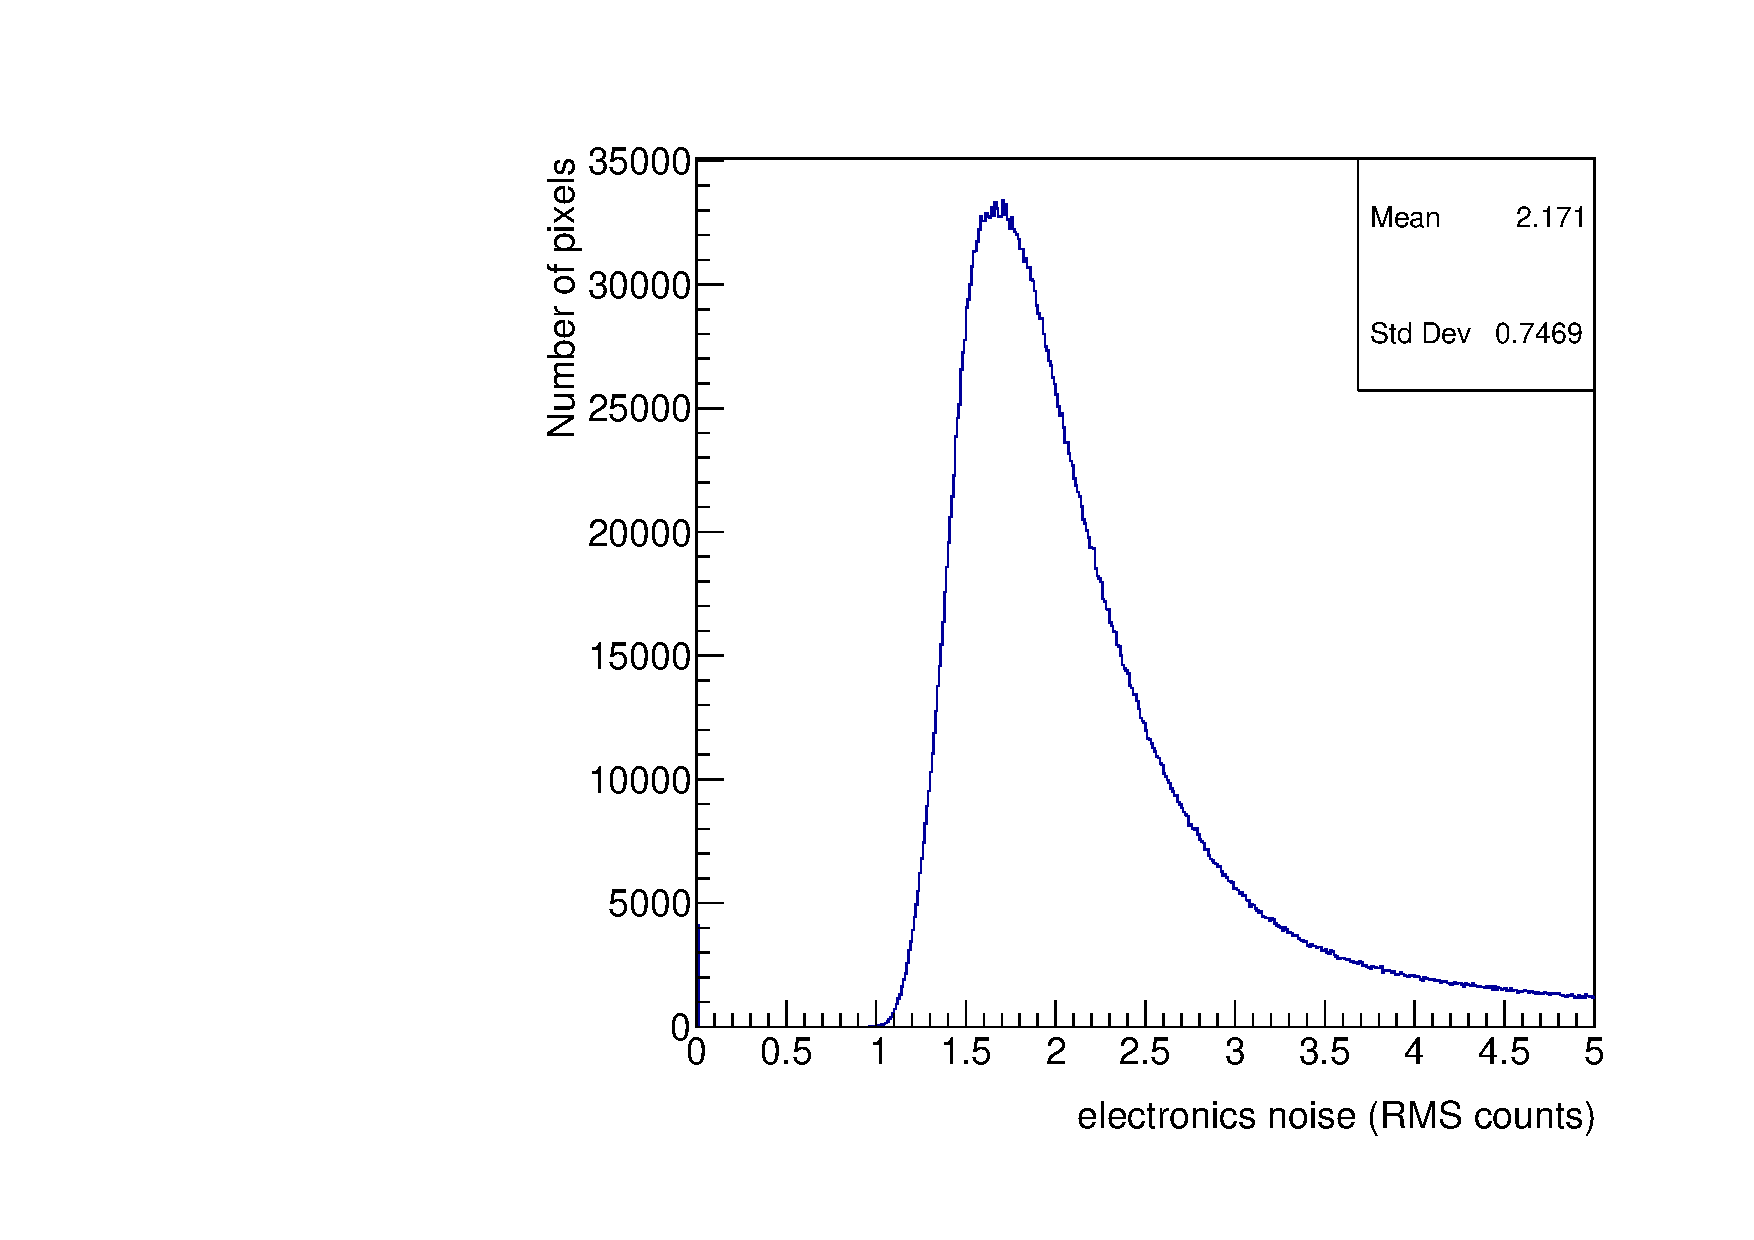
\includegraphics[width=0.45\linewidth]{figures/sensor_noise}
  \caption{Distribution of the electronic noise of the sensor,
    estimated in images taken with sensor in complete dark, and
    evaluated as the SD of the distribution of the counts for each
    pixel.  \label{fig:noise}}
\end{figure}
%
On such pedestal-subtracted zero-suppressed images an upper threshold
was applied to reject hot pixels, which are more likely due to sensor
instabilities than to a real energy release. They are found to be not
malfunctioning pixels since they disappear after a power cycle of the
camera: therefore a dynamic (run-by-run) suppression is needed.  They
are efficiently identified as high-intensity, isolated pixels, and
distinguished by a true energy deposit, for which each pixel is
surrounded by some other active pixels. A threshold is applied on the
ratio $R_9$ between the pixel and the average of the counts in a
$3{\times}3$ pixels matrix surrounding it, and a minimum number of two
pixels above noise in that matrix is required to discriminate good
pixels from hot ones. Only good pixels are retained for the subsequent
clustering.

The resolution of the resulting image is initially reduced by forming
\textit{macro-pixels}, by averaging the counts in $4{\times}4$ pixel
matrices. This is needed to reduce the combinatorics of the subsequent
clustering algorithm, in order to be executed in a reasonable time for
each image. On such $512{\times}512$ pixel map, a median
filter~\cite{medianfilter} is applied, which is effective in
suppressing the electronics noise fluctuations in a $4{\times}4$ pixel
matrix and it is computationally efficient, as described in more
details in Ref.~\cite{medianfilter_cygno}. The output image is passed
to the basic clustering algorithm, described in the following.


